% TeXstudio spellcheck 2020-12-10 16:38

\chapter{Tesztgenerálás megvalósítása Theta környezetben} \label{main-gyakorlat}

Ebben a fejezetben bemutatom \aref{theta}. fejezetben ismertetett, Java nyelven írt Theta  modellellenőrző keretrendszer meglévő, felhasznált komponenseit (\ref{theta-felhasznalt}. fejezet), majd részletesen bemutatom \aref{main-elmelet}. fejezetben leírt tesztgenerálási algoritmus megvalósítását (\ref{megvalositas}. fejezet).

\section{A Theta meglévő, felhasznált komponensei} \label{theta-felhasznalt}

A megvalósítás során felhasználtam a Theta számos meglévő, modellellenőrzéshez használt komponensét. Ezen komponensek bemutatása során csak azokra a részekre térek ki, amelyek a szakdolgozat szempontjából relevánsak.

Az átláthatóság végett az UML osztálydiagramokon alapvetően nem jelöltem a getter és setter függvényeket, hanem ezek megléte esetén publikusként jelöltem az adattagot magát. Ettől csak ott tértem el, ahol a különbség releváns, pl. ha az absztrakt getter már az ősosztályban szerepel, majd a leszármazott osztály definiálja. A diagramokon a $\oplus$ jel jelöli a beágyazott osztályt.

\subsection{XtaCli}
Az \textsf{XtaCli} osztály az XTA formalizmushoz biztosít egyszerű parancssoros interfészt. A futása parancssori paraméterekkel konfigurálható, mint pl. a modellt tartalmazó fájl neve, választott bejárási stratégiák stb.

A \textsf{main} függvény példányosítja az \textsf{XtaCli} osztályt, majd meghívja a \textsf{run} metódusát, ahol az érdemi működés található.

A \textsf{loadModel} metódus a paraméterként kapott fájlból az \textsf{XtaDslManager} osztály \textsf{createSystem} statikus metódusával beolvassa a rendszert leíró XTA fájlt, és létrehoz belőle egy \textsf{XtaSystem} objektumot.

Ezt követően a \textsf{LazyXtaCheckerFactory} osztály statikus \textsf{create} függvénye létrehoz egy \textsf{SafetyChecker} objektumot, melynek a \textsf{check} metódusa elvégzi az \textsf{XtaSystem} objektum modellellenőrzését, ami egy \textsf{SafetyResult} objektumot ad eredményül. Ebben az objektumban található a \textsf{getArg} metódussal elérhető \textsf{ARG} objektum, amely a rendszer absztrakt elérhetőségi gráfja \emph{(Abstract Reachability Graph)}.

\subsection{XtaSystem}
\begin{figure}%[h!]
    \centering
    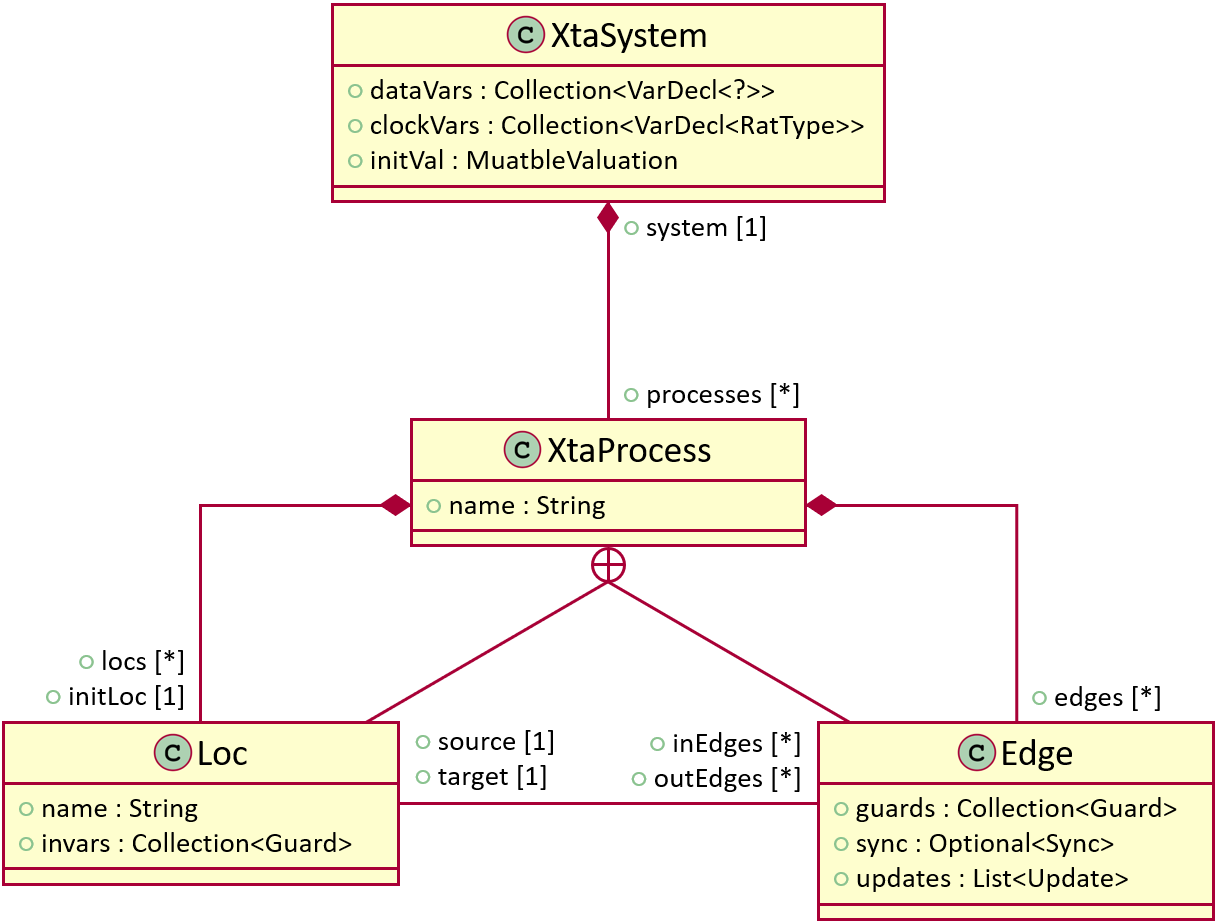
\includegraphics[height=100mm, keepaspectratio]{src/figures/xtasystem-uml.png}
    \caption{Az \textsf{XtaSystem}, \textsf{XtaProcess}, \textsf{Loc}, és \textsf{Edge} osztályok UML osztálydiagramja}
    \label{fig:xtasystem-uml}
\end{figure}

Az \textsf{XtaSystem} osztály időzítettautomata-hálózatok leírására alkalmas, vagyis egy példánya időzített automaták egy $\automatanetwork$ hálózatát írja le. Itt találhatók a hálózat óraváltozói (\textsf{clockVars : Collection<VarDecl<RatType>{}>}) és adatváltozói (\textsf{dataVars : Collection<VarDecl<?>{}>}), utóbbiak kezdeti értékei (\textsf{initVal : MutableValuation}), valamint a hálózatot alkotó $\automatanetwork_i$ időzített automata példányok (\textsf{processes : List<XtaProcess>}).

Az \textsf{XtaProcess} osztály példányai időzített automatákat írnak le. Egy \textsf{XtaProcess} példány rendelkezik névvel (\textsf{name : String}), ismeri az őt tartalmazó hálózatot (\textsf{system : XtaSystem}), valamint tartalmazza a vezérlési helyeit (\textsf{locs : Collection<Loc>}), az éleit (\textsf{edges : Collection<Edge>}) és a kezdő vezérlési helyét (\textsf{initLoc : Loc}).

Az \textsf{XtaProcess} beágyazott osztályai a vezérlési helyeket reprezentáló \textsf{Loc}, valamint az éleket reprezentáló \textsf{Edge}.

Egy \textsf{Loc} objektum tárolja a vezérlési hely nevét (\textsf{name : String}), a belé vezető éleket (\textsf{inEdges : Collection<Edge>}), a belőle kivezető éleket (\textsf{outEdges : Collection<Edge>}), valamint a vezérlési hely invariánsait (\textsf{invars : Collection<Guard>}).

Egy \textsf{Edge} objektum tárolja az él forrás (\textsf{source : Loc}) és cél (\textsf{target : Loc}) vezérlési helyét, az őrfeltételeit (\textsf{guards : Collection<Guard>}), a szinkronizációját (\textsf{sync : Optional<Sync>}) és a változókon végzett frissítéseit (\textsf{updates : List<Update>}).

Az \textsf{XtaSystem}, \textsf{XtaProcess}, \textsf{Loc}, és \textsf{Edge} osztályok UML osztálydiagramja a \ref{fig:xtasystem-uml}. ábrán látható.

\subsection{ARG}
\begin{figure}%[h!]
    \centering
    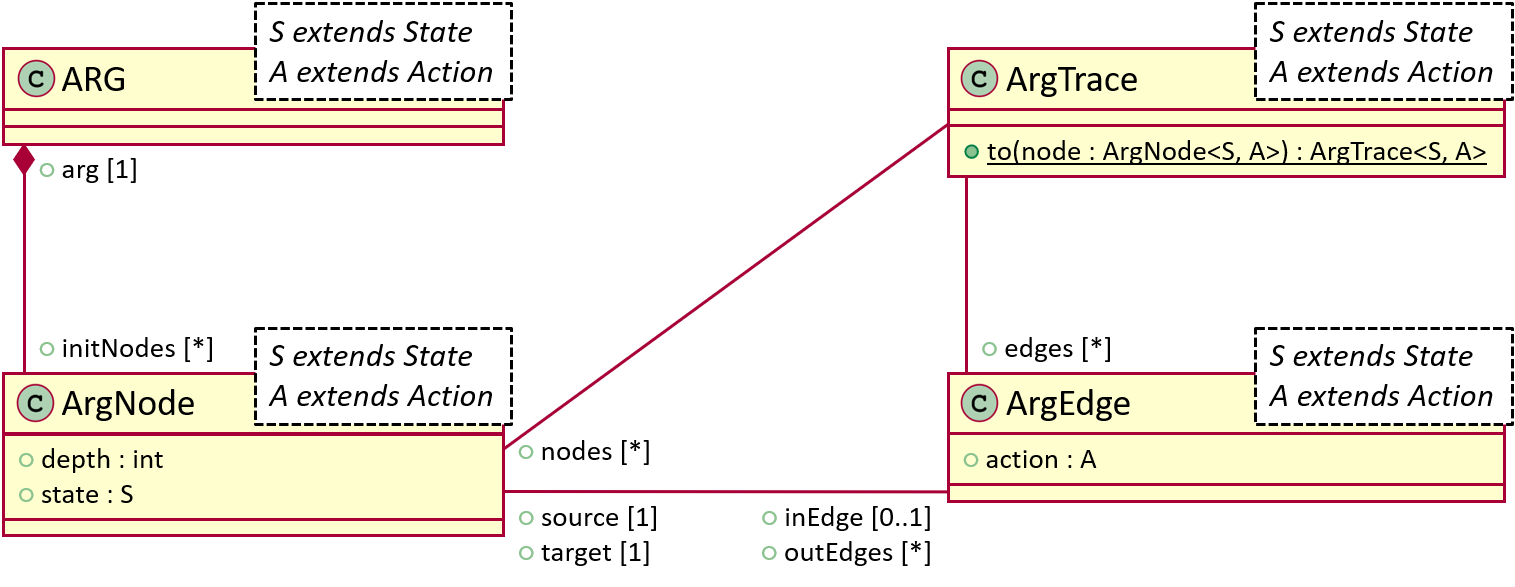
\includegraphics[width=\textwidth, keepaspectratio]{src/figures/arg-uml.png}
    \caption{Az \textsf{ARG}, \textsf{ArgNode}, \textsf{ArgEdge}, és \textsf{ArgTrace} osztályok UML osztálydiagramja}
    \label{fig:arg-uml}
\end{figure}

Egy \textsf{ARG} példány egy absztrakt elérhetőségi gráfot reprezentál. Ez megegyezik a \ref{Theta:felepites}. fejezetben említett ART-vel (absztrakt elérhetőségi fa), és megvalósítja a \ref{def:ASG}. definícióban (ASG) leírtakat.

\textsf{ARG<S extends State, A extends Action>} egy generikus osztály, melynek két típusparamétere az \textsf{S} állapot- és \textsf{A} akciótípus. Esetünkben az \textsf{S} típusparaméter az \textsf{XtaState}, az \textsf{A} típusparaméter pedig az \textsf{XtaAction} lesz. 

Egy \textsf{ARG} gráf \textsf{ArgNode} típusú csúcsokból és \textsf{ArgEdge} típusú élekből áll, de az \textsf{ARG} csak a kezdő csúcsait (\textsf{initNodes : Collection<ArgNode<S, A>{}>}) ismeri közvetlenül.

Egy \textsf{ARG<S, A>} egy hasonlóan generikus \textsf{ArgNode<S, A>} csúcsa ismeri az őt tartalmazó gráfot (\textsf{arg : ARG<S, A>}), tárolja a saját mélységét a fában (\textsf{depth : int}), a belé vezető élt (\textsf{inEdge : Optional<ArgEdge<S, A>{}>}) és a belőle kivezető éleket (\textsf{outEdges : Collection<ArgEdge<S, A>{}>}), valamint a csúcs állapotát (\textsf{state : S}).

Egy \textsf{ARG<S, A>} egy hasonlóan generikus \textsf{ArgEdge<S, A>} éle tárolja forrás (\textsf{source : ArgNode<S, A>}) és cél (\textsf{target : ArgNode<S, A>}) csúcsát, valamint az él akcióját (\textsf{action : A}).

Az \textsf{ArgTrace<S extends State, A extends Action>} osztály egy \textsf{ARG}-beli utat reprezentál, vagyis csúcsok (\textsf{nodes : List<ArgNode<S, A>{}>}) és élek (\textsf{edges : List<ArgEdge<S, A>{}>}) alternáló sorozatát. Az \textsf{ArgTrace} osztály statikus \textsf{to} metódusa a paraméterként kapott \textsf{ArgNode} csúcshoz vezető \textsf{ArgTrace}-t ad vissza.

Az \textsf{ARG}, \textsf{ArgNode}, \textsf{ArgEdge}, és \textsf{ArgTrace} osztályok UML osztálydiagramja a \ref{fig:arg-uml}. ábrán látható.

\subsection{XtaState}

\begin{figure}%[h!]
    \centering
    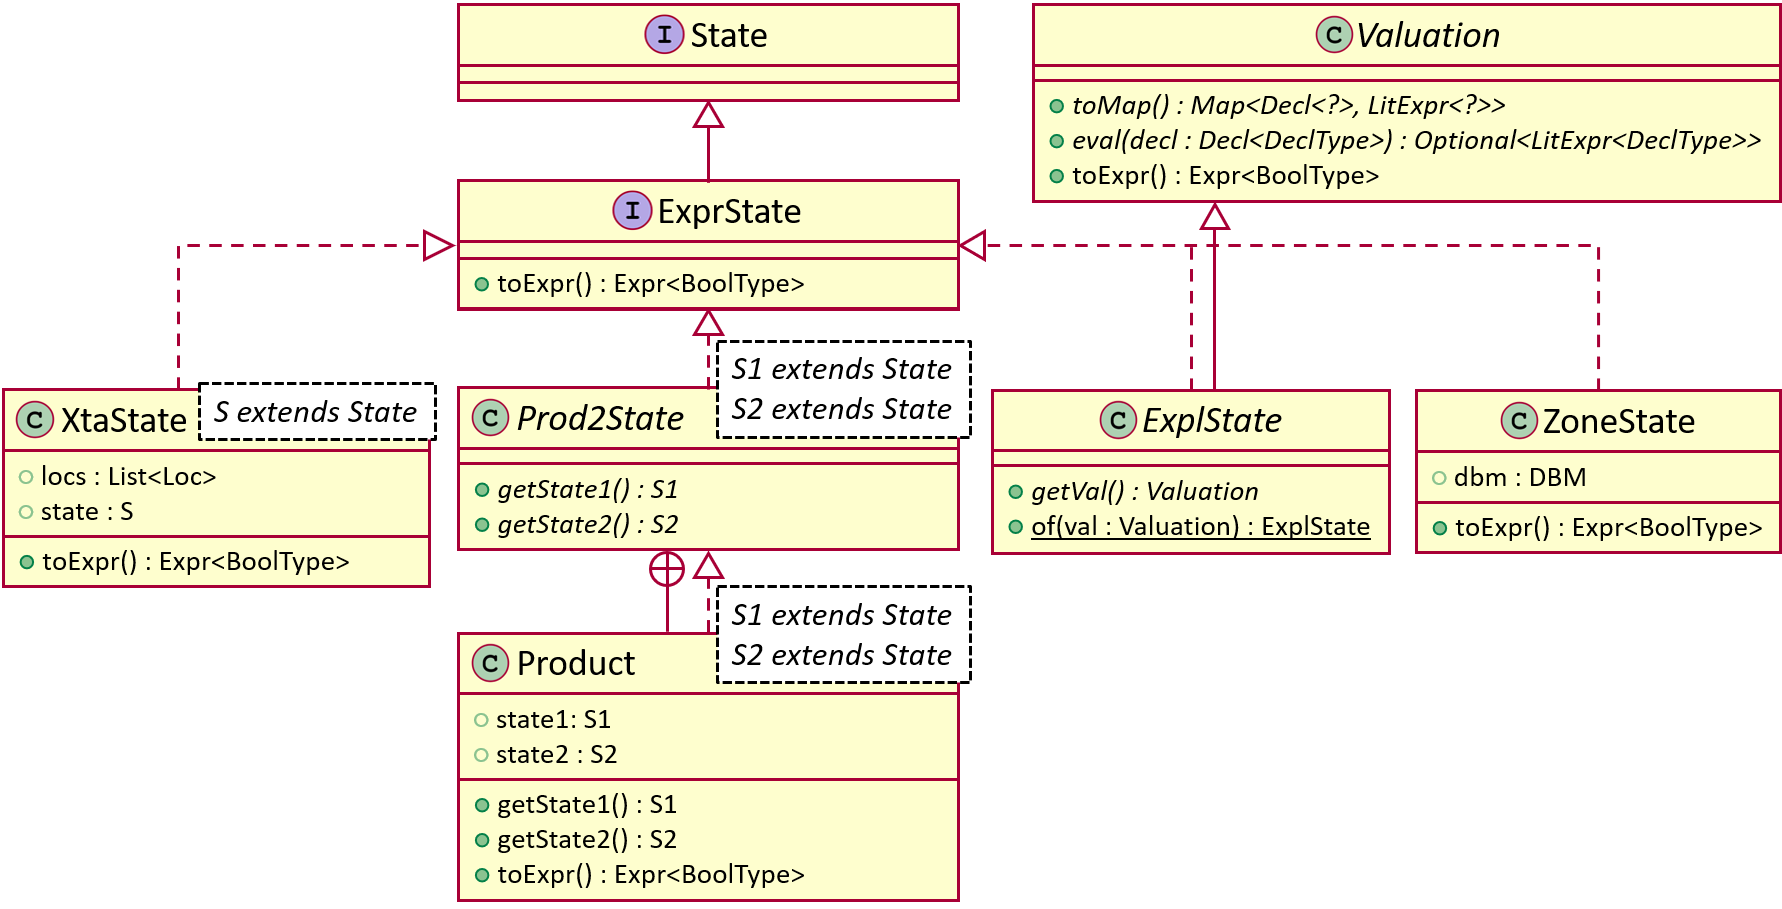
\includegraphics[width=\textwidth, keepaspectratio]{src/figures/xtastate-uml.png}
    \caption{Az \textsf{XtaState} és kapcsolódó osztályok UML osztálydiagramja}
    \label{fig:xtastate-uml}
\end{figure}

Az \textsf{XtaState<S extends State>} generikus osztály egy \textsf{ArgNode} állapotát írja le. Tárolja az állapotban aktív vezérlési helyeket (\textsf{locs : List<Loc>}), valamint egy állapotot (\textsf{state : S}), amely esetünkben két állapot szorzata (\textsf{Prod2State.Product}). Az állapotot ugyanis egy explicit állapot (\textsf{ExplState}) és egy zónaállapot (\textsf{ZoneState}) együtt határozzák meg. Előbbi az értékváltozókra vonatkozó kényszereket (\textsf{Valuation} alakban), míg utóbbi a zónákat, vagyis az óraváltozókra vonatkozó kényszereket (\textsf{DBM} alakban) tartalmazza.

Az imént említett osztályok (\textsf{XtaState}, \textsf{Prod2State.Product}, \textsf{ExplicitState}, \textsf{ZoneState}) mind megvalósítják az \textsf{ExprState} interfészt, vagyis definiálniuk kell a \textsf{toExpr} függvényt. Ez a függvény az objektumban lévő kényszereket egy \textsf{Expr<BoolType>} objektummá alakítja.

Az \textsf{XtaState} és kapcsolódó osztályok UML osztálydiagramja a \ref{fig:xtastate-uml}. ábrán látható.

\subsection{XtaAction}
\begin{figure}%[h!]
    \centering
    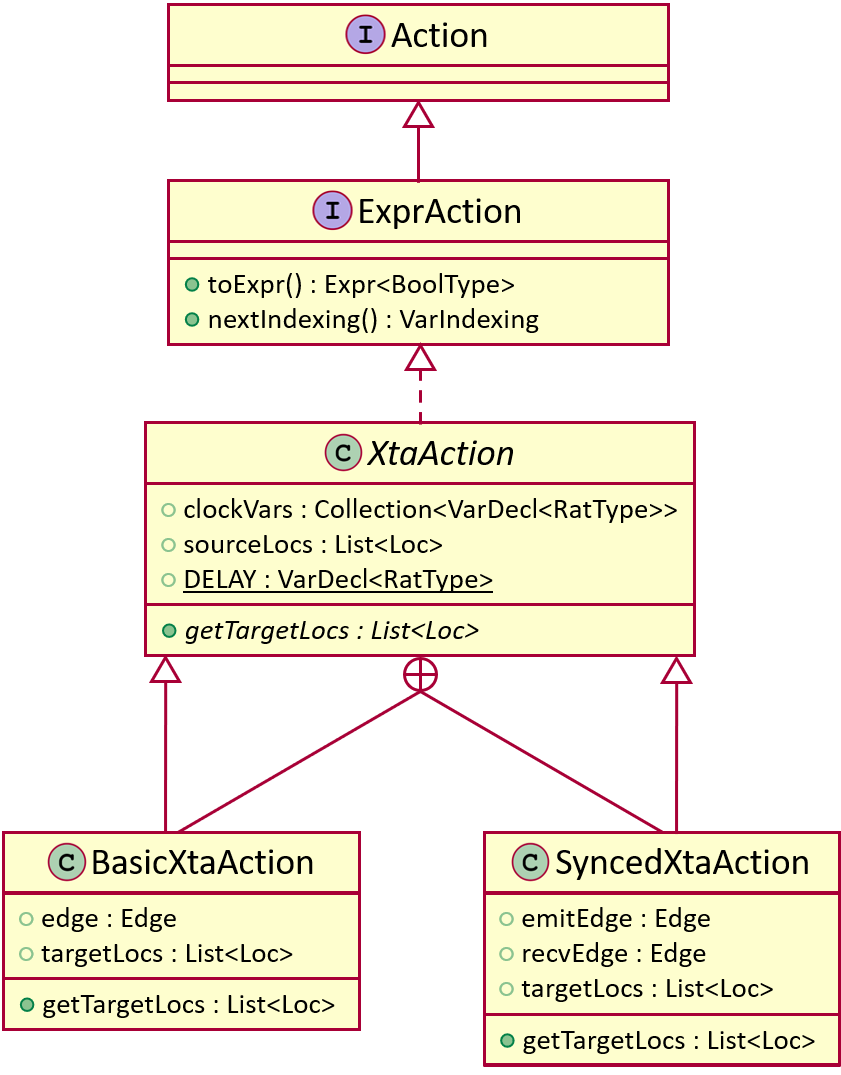
\includegraphics[height=120mm, keepaspectratio]{src/figures/xtaaction-uml.png}
    \caption{Az \textsf{XtaAction} és kapcsolódó osztályok UML osztálydiagramja}
    \label{fig:xtaaction-uml}
\end{figure}

Az \textsf{XtaAction} osztály egy \textsf{ArgEdge} akcióját írja le. Ismeri az óraváltozókat (\textsf{clockVars : Collection<VarDecl<RatType>{}>}), illetve a forrás (\textsf{sourceLocs : List<Loc>}) és cél (\textsf{targetLocs : List<Loc>}) állapotban aktív vezérlési helyeket. Itt található továbbá a statikus, \textsf{VarDecl<RatType>} típusú \textsf{DELAY} adattag, amely azt a változót reprezentálja, amely megadja, hogy egy állapotban mennyit várakozik a rendszer.

Az \textsf{XtaAction} osztály absztrakt, két leszármazottal: a \textsf{BasicXtaAction} osztály szinkronizáció nélküli átmeneteket, míg a \textsf{SyncedXtaAction} osztály szinkronizáló átmeneteket reprezentál. A \textsf{BasicXtaAction} osztály egy időzített automata egyetlen élére (\textsf{edge : Edge}) vonatkozik, míg a \textsf{SyncedXtaAction} osztály egyaránt ismeri a szinkronizációt küldő (\textsf{emitEdge : Edge}) és fogadó (\textsf{recvEdge : Edge}) élt.

Az \textsf{XtaState}-nél bemutatotthoz hasonlóan az \textsf{XtaAction} is megvalósítja az \textsf{ExprAction} interfészt, vagyis definiálja az ott deklarált \textsf{toExpr} metódust. Ennek a működése megegyezik az \textsf{ExprState}-nél leírttal.

\subsection{Típusok}

\begin{figure}%[h!]
    \centering
    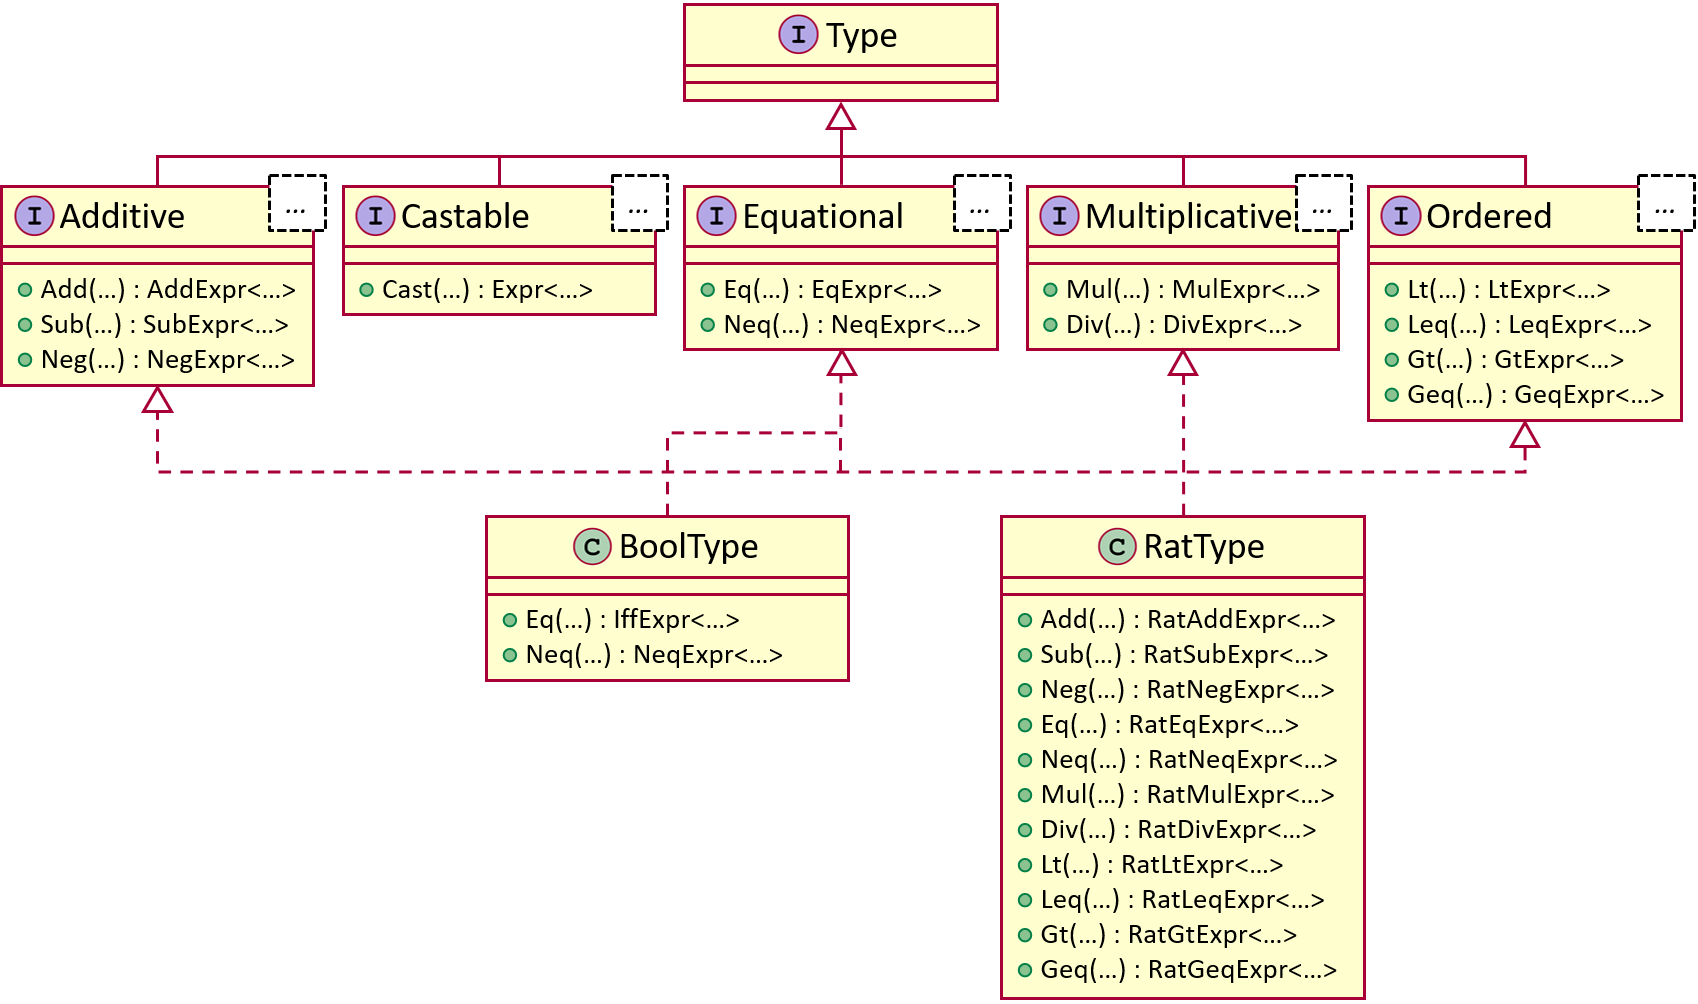
\includegraphics[width=\textwidth, keepaspectratio]{src/figures/type-uml.png}
    \caption{Típusok a Theta-ban}
    \label{fig:type-uml}
\end{figure}

A Theta típusainak őse a \textsf{Type} interfész. Ezt valósítják meg az \textsf{Additive}, \textsf{Castable}, \textsf{Equational}, \textsf{Multiplicative} és \textsf{Ordered} interfészek (értelemszerű függvénydeklarációkkal), amelyek implementálása azt jelenti, hogy az adott típuson értelmezhetők a névben szereplő műveletek (összeadás, kivonás, negálás; típuskonverzió; egyenlőségvizsgálat; szorzás, osztás; összehasonlítás).

A \textsf{BoolType} a logikai típust, a \textsf{RatType} a racionális típust jelöli. Ezen osztályok egyszerűsített UML osztálydiagramja látható a \ref{fig:type-uml}. ábrán.

\subsection{Változók}
\begin{figure}%[h!]
    \centering
    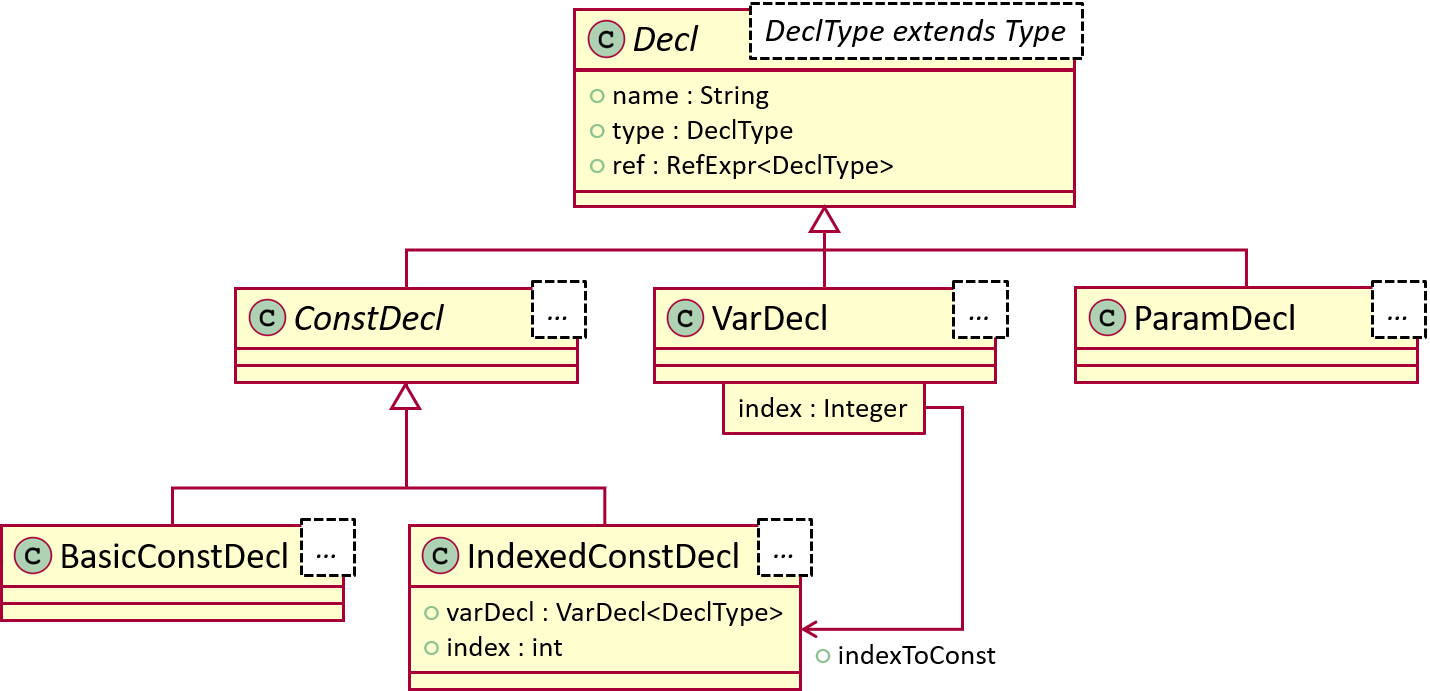
\includegraphics[width=\textwidth, keepaspectratio]{src/figures/decl-uml.png}
    \caption{Deklarációk a Theta-ban}
    \label{fig:decl-uml}
\end{figure}

A Theta-ban háromféle dolgot deklarálhatunk: konstanst, változót és paramétert. Minden deklaráció a generikus \textsf{Decl<DeclType extends Type>} ősből származik, amely tartalmazza a deklaráció nevét (\textsf{name : String}), típusát (\textsf{type : DeclType}) és referenciáját (\textsf{ref : RefExpr<DeclType>}). Minden \textsf{Decl}-ből leszármazó specifikus deklaráció is \textsf{Decl}-lel megegyezően generikus.

Kétféle konstansdeklaráció lehetséges: \textsf{BasicConstDecl} és \textsf{IndexedConstDecl}. Utóbbi egy változó adott indexelésére vonatkozik, ennek megfelelően egy változódeklarációt (\textsf{varDecl : VarDecl<DeclType>}) és egy indexet (\textsf{index : int}) tartalmaz.

A változódeklaráció (\textsf{VarDecl}) tartalmaz egy hozzárendelést (\textsf{indexToConst : Map<Integer, IndexedConstDecl<DeclType>{}>}), amely egy indexeléséhez egy indexelt konstansdeklarációt rendel.

A \textsf{VarIndexing} osztály változókhoz rendel indexértékeket, így alkalmas annak a tárolására, hogy egy kifejezésben melyik változó milyen indexszel szerepel. Az alapértelmezett \textsf{defaultIndex : int} indexhez képest tárolja a változók indexeltolását (offszet) a \textsf{varToOffset : Map<VarDecl<?>, Integer>}-ben. A \textsf{get} függvény adja meg egy adott \textsf{varDecl} változóhoz tartozó indexet, melynek visszatérési értéke \textsf{defaultIndex} és \textsf{varDecl} \textsf{varToOffset}-ben tárolt offszetjének összege.

A deklarációkat leíró osztályok UML osztálydiagramja látható a \ref{fig:decl-uml}. ábrán.

\subsection{Kifejezések}

\begin{figure}%[h!]
    \centering
    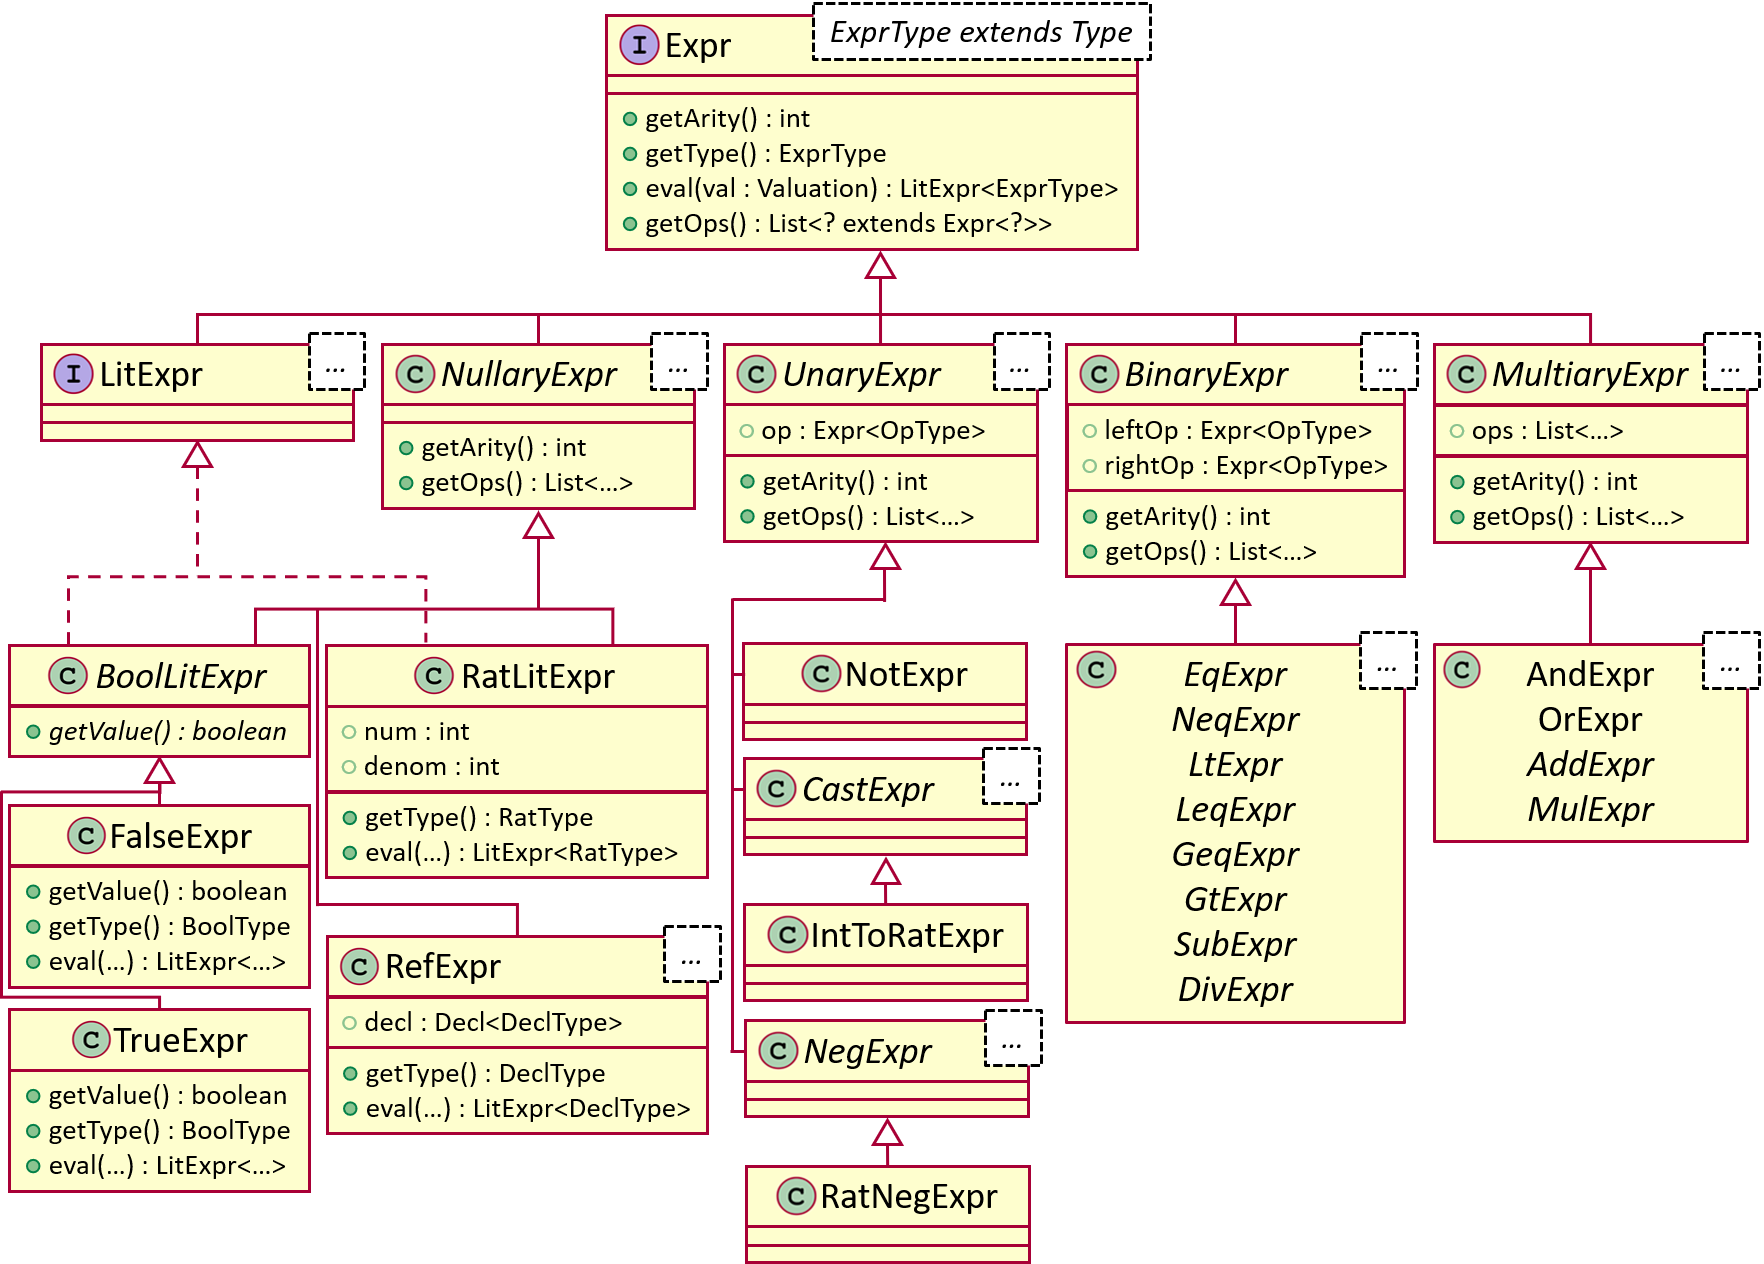
\includegraphics[width=\textwidth, keepaspectratio]{src/figures/expr-uml.png}
    \caption{Kifejezések a Theta-ban}
    \label{fig:expr-uml}
\end{figure}

A Theta kifejezéseinek őse a generikus \textsf{Expr} interfész, melynek \textsf{ExprType extends Type} típusparamétere a kifejezés értékének típusa. A kifejezés típusát a \textsf{getType}, aritását a \textsf{getArity}, operandusait a \textsf{getOps} metódus adja meg. A kifejezés kiértékelésére az \textsf{eval} metódus szolgál, melynek \textsf{Valuation} típusú \textsf{val} paramétere deklarációkhoz rendel literál kifejezéseket, visszatérési értéke pedig kifejezés értékét reprezentáló literál. A \textsf{val} paraméter hordozza az információt, hogy a kifejezésben található deklarációreferencia változók (\textsf{RefExpr}) helyére milyen literál értéket (\textsf{LitExpr}) kell behelyettesíteni.

Az \textsf{Expr} interfészt megvalósító absztrakt osztályok a kifejezések aritása szerinti ősosztályok (\textsf{NullaryExpr}, \textsf{UnaryExpr}, \textsf{BinaryExpr}, \textsf{MultiaryExpr}), ezekből származnak le a konkrét műveleteket reprezentáló kifejezésosztályok (típusspecifikus műveletek esetén (pl. negálás: \textsf{NegExpr}) ebből még további típusspecifikus osztályok származnak le (pl. racionális negálás: \textsf{RatNegExpr})).

A 0 aritású kifejezések lehetnek literálok, vagyis típusspecifikus értékek, vagy deklarációreferenciák, vagyis egy deklaráció konkrét használati esetei. Egy deklarációreferencia által referált deklarációhoz egy \textsf{Valuation} objektum rendel literál értéket az \textsf{eval} metódusával.

A \textsf{PathUtils} osztály statikus \textsf{unfold} metódusa egy \textsf{expr : Expr} kifejezést és egy \textsf{varIndexing : VarIndexing} változóindexelést kap paraméterül. A visszatérési értéke egy olyan kifejezés, amelyben az \textsf{expr}-beli \textsf{VarDecl}-re referáló \textsf{RefExpr}-ek a megfelelő \textsf{varIndexing}-beli indexszel vannak indexelve.

A kifejezéseket bemutató egyszerűsített UML osztálydiagram a \ref{fig:expr-uml}. ábrán látható. A \textsf{BinaryExpr} és \textsf{MultinaryExpr} osztályok ősei a könnyebb áttekinthetőség érdekében tömörítve láthatók, a további típusspecifikus leszármazottak nem szerepelnek az ábrán.

\subsection{Solver}
A Theta által használt SMT megoldók a \textsf{Solver} interfészen keresztül érhetők el. Az \textsf{add} függvénnyel adhatunk meg új, \textsf{Expr<BoolType>} típusú kényszereket. A \textsf{pop} metódus eltávolítja a legutóbbi \textsf{push} óta hozzáadott kényszereket.

A \textsf{check} metódus megvizsgálja a probléma kielégíthetőségét, amit egy \textsf{SolverStatus} enumként ad vissza, amelynek az \textsf{isSat} metódusa megadja a kielégíthetőség logikai értékét.

Amennyiben a probléma kielégíthető, a \textsf{getModel} metódus megadja azt a \textsf{Valuation} objektumot, amely tartalmazza a megoldott SMT probléma változóinak értékeit, vagyis a probléma megoldását.

\subsection{Vizualizáció}
A Theta egyaránt támogatja belső gráfreprezentációk kiírását dot formátumba, illetve közvetlen kirajzolását számos kiterjesztésű képfájlba a Graphviz\footnote{\url{http://www.graphviz.org/}} eszközzel.

A Theta belső gráfreprezentációja a \textsf{Graph} osztály, amely egy azonosítóval (\textsf{id : String}), címkével (\textsf{label : String}), valamint csúcsokkal (\textsf{nodes : Map<String, Node>}) és élekkel (\textsf{edges : Collection<Edge>}) rendelkezik. Az \textsf{addNode} metódus egy új csúcsot ad hozzá a gráfhoz, egyedi azonosítóval (\textsf{id : String}) és tetszőleges attribútumokkal (\textsf{attributes : NodeAttributes}). Az \textsf{addEdge} metódus élt ad hozzá a gráfhoz két adott azonosítójú (\textsf{sourceId, targetId : String}) csúcs közé, tetszőleges attribútumokkal (\textsf{attributes : EdgeAttributes}).

Az attribútum osztályokban (\textsf{NodeAttributes, EdgeAttributes}) található tulajdonságok megfeleltethetők a dot nyelvben lévő csúcs- és éltulajdonságoknak.\footnote{\url{https://www.graphviz.org/pdf/dotguide.pdf}} Egy tetszőleges gráf előállításához tehát csupán megfelelő \textsf{NodeAttributes} és \textsf{EdgeAttributes} objektumokat kell átadnunk egy \textsf{Graph} objektum \textsf{addNode} és \textsf{addEdge} függvényének.

Egy \textsf{Graph} objektumot a \textsf{GraphvizWriter} osztály \textsf{writeFile} függvényével írhatunk ki számos formátumú fájlba. A függvény paraméterlistája egy \textsf{Graph} objektumból, a kimeneti fájl nevéből és egy fájlformátumot leíró \textsf{GraphvizWriter.Format} enumból áll.

\subsection{Logger}
A Theta beépítetten támogatja a naplózást (logolást) is, a \textsf{Logger} interfészen keresztül. A \textsf{Logger.Level} enummal határozható meg az adott logolás prioritása. A \textsf{write} metódus segítségével írhatunk a logba, adott prioritással.

\section{A tesztgenerálás megvalósítása} \label{megvalositas}

A tesztgenerálás megvalósítására külön alprojektet (\textsf{xta-testgeneration}) és package-et (\textsf{hu.bme.mit.theta.xta.testgeneration}) hoztam létre.

Az \textsf{XtaCli} osztályt kiegészítettem egy további parancssori kapcsoló (\texttt{-{}-testgen} vagy \texttt{-t}) kezelésével (\textsf{testGeneration}). Amennyiben ezzel indítják a programot, a \textsf{run} metódus meghívja a \textsf{XtaTestGenerator} osztály \textsf{generateTests} metódusát, amely egy időzített teszttel (\textsf{Set<? extends XtaTest<?, ?>{}>}) tér vissza.

Ezt a tesztkészletet ezután a \textsf{printTests} metódussal kiíratjuk a konzolra, a \textsf{visualizeTests} metódussal pedig kirajzoltatjuk fájlokba. Előbbi az \textsf{XtaTestPrinter}, utóbbi az \textsf{XtaTestVisualizer} osztályt használja.

\subsection{XtaTest}
Az \textsf{XtaTest<S extends XtaState<? extends State>, A extends XtaAction>} osztály egy példánya reprezentál egy időzített tesztesetet. Egy tesztesetet egy név (\textsf{name : String}), egy ARG-beli útvonal (\textsf{trace : ArgTrace<S, A>}), valamint az időzítések (\textsf{delays : List<Double>}) határoznak meg. A \textsf{getTotalTime} metódus megadja a \textsf{delays}-beli várakozások összegét, a \textsf{getLocs} metódus pedig a teszt által érintett vezérlési helyek halmazát.

\subsection{XtaTestGenerator}
A tesztgenerálást egy \textsf{XtaSystem} objektum által leírt $\automatanetwork$ automatahálózathoz egy \textsf{ARG} objektum alapján az \textsf{XtaTestGenerator} osztály végzi, egy \textsf{Solver} és egy \textsf{Logger} objektum felhasználásával.

A \textsf{generateTests} metódus valósítja meg az \ref{GenerateTests}. algoritmust, vagyis szélességi bejárással addig generál új teszteket (\textsf{generateTest}), amíg a $\networktestset$ tesztkészlet le nem fedi az $\automatanetwork$ automatahálózat összes vezérlési helyét.

A \textsf{generateTest} metódus az ARG egy konkrét csúcsához vezető $\networktest$ tesztesetet generál a \ref{GenerateTest}. algoritmusban leírtak szerint. A paraméterként kapott \textsf{ArgNode}-hoz az \textsf{ArgTrace} osztály statikus \textsf{to} metódusával generál \textsf{ArgTrace}-t. A generált útvonalú teszteset időzítését a \textsf{calculateDelays} metódus végzi.

A \textsf{calculateDelays} metódus valósítja meg a \ref{CalculateDelays}. algoritmusban leírtakat, vagyis egy $\networktest$ tesztesetnek kiszámolja a $\hat{t}(\networktest)$ időzítését. Először összeállítja a megoldandó SMT problémát, majd megoldja azt a \textsf{Solver} objektum felhasználásával, végül megkísérli javítani a kapott megoldást. A problémát adó kényszerek a következő metódushívásokkal állnak elő:
\begin{enumerate}
    \item \textsf{addInitialClockConstraint}: a kezdő várakozások meg kell, hogy egyezzenek az óraváltozók kezdeti értékével,
    \item \textsf{addInitialNodeConstraint}: a kezdőállapotot leíró kényszerek,
    \item \textsf{addTraceConstraints}: a teszteset éleit és újabb állapotait leíró kényszerek,
    \item \textsf{addSumOfDelaysConstraint}: új változó deklarálása $time(\networktest) = \sum\limits_{i = 1}^{|\networktest|} \hat{t}_i$-re.
\end{enumerate}

Az \textsf{addInitialClockConstraints} függvény az \textsf{XtaSystem} objektum \textsf{getClockVars} metódusával lekéri $\automatanetwork$ összes óraváltozóját, valamint létrehoz egy \textsf{delayRef : RefExpr<RatType>} referenciát az \textsf{XtaAction} osztály statikus \textsf{DELAY} változójára. Végigiterál az összes \textsf{cv} óraváltozón, létrehoz rájuk egy \textsf{clockVarRef : RefExpr<RatType>} referenciát a \textsf{RefExpr} osztály statikus \textsf{to} függvényével, majd egy listába teszi a \textsf{delayRef} és \textsf{clockVarRef} közti egyenlőség kifejezéseket, amelyeket az \textsf{EqExpr} osztály statikus \textsf{create2} függvényével hoz létre. Az \textsf{AndExpr} osztály statikus \textsf{to} függvényével ÉS kapcsolatba fűzi az imént létrehozott egyenlőség kifejezéseket, majd a \textsf{PathUtils} osztály statikus \textsf{unfold} függvényével minden változót 0-val indexel. Az így kapott \textsf{Expr<BoolType>} kifejezést adja hozzá a \textsf{Solver} objektumhoz.

Az \textsf{addInitialNodeConstraint} függvény a paraméterként kapott \textsf{ArgTrace} objektum kezdő \textsf{ArgNode}-jának állapotát alakítja \textsf{Expr<BoolType>} objektummá a \textsf{toExpr} metódus segítségével, majd a kifejezés változóit 0-val indexeli a \textsf{PathUtils} osztály \textsf{unfold} függvényével. Az így kapott \textsf{Expr<BoolType>} kifejezést adja hozzá a \textsf{Solver} objektumhoz.

Az \textsf{addTraceConstraints} függvény végigiterál a paraméterként kapott \textsf{ArgTrace} objektum további csúcsain és élein, és azok \textsf{XtaState} állapotát illetve \textsf{XtaAction} élét azok \textsf{toExpr} metódusával \textsf{Expr<BoolType>} kifejezéssé alakítja. Ezen kifejezések megfelelően indexelt alakját adja hozzá a \textsf{Solver} objektumhoz. A megfelelő indexelés megállapításához a paraméterként kapott \textsf{indexing : List<VarIndexing>} listához mindig hozzáad egy újabb elemet, amelyet úgy kap meg, hogy a legutóbbi \textsf{VarIndexing} elemhez hozzáadja az \textsf{XtaAction} objektum \textsf{nextIndexing} metódusa által visszaadott indexelést.

Az \textsf{addSumOfDelays} függvény egy új \textsf{totalTime : ConstDecl<RatType>} racionális típusú deklarációt hoz létre \texttt{\_\_total\_\_time\_\_} névvel, illetve egy erre mutató \textsf{totalTimeRef : RefExpr<RatType>} referenciát. Az \textsf{XtaAction} osztály statikus \textsf{DELAY} adattagjára is létrehoz egy \textsf{delayRef : RefExpr<RatType>} referenciát. Ezután összegyűjti a teszt összes lépéséhez tartozó \textsf{delayRef}-indexelést a \textsf{delayRefs : List<Expr<RatType>{}>} listába a \textsf{PathUtils} osztály statikus \textsf{unfold} függvényének segítségével. Végül hozzáadja a \textsf{Solver} objektumhoz a \textsf{delayRefs}-beli elemek összegének és \textsf{totalTimeRef}-nek az egyenlőségét az \textsf{EqExpr} és \textsf{AddExpr} osztályok statikus \textsf{create2} függvényének segítségével.

Miután a \textsf{Solver} objektum megoldást talált a \textsf{calculateDelays} által összeállított problémára, a \textsf{reduceDelays} megkísérli javítani azt $time(\networktest)$ csökkentésével.

A \textsf{reduceDelays} metódus addig szorítja egyre szűkebb \textsf{min, max : RatLitExpr} korlátok közé \textsf{totalTime} értékét, amíg az intervallum már olyan szűk, hogy nincs értelme további javítási próbálkozásnak. Az alsó \textsf{min} korlát kezdetben 0, míg a felső \textsf{max} korlát kezdetben az eredeti időzítés \textsf{totalTime} értéke.

A ciklus minden lépésben \textsf{min} és \textsf{newMax} közé próbálja szorítani a teszt teljes idejét egy \textsf{totalTime} $\leq$ \textsf{newMax} kényszer hozzáadásával. \textsf{newMax} értéke minden esetben a \textsf{min} és \textsf{max} által meghatározott intervallum közepe, vagyis \textsf{min} $+$ (\textsf{max} $-$ \textsf{min}) $/ 2$.

Amennyiben van \textsf{newMax}-nál kisebb megoldás, \textsf{max} új értéke az új megoldás \textsf{totalTime} értéke lesz, amennyiben pedig nincs, \textsf{min} új értéke lesz \textsf{newMax} előző értéke. \textsf{newMax} értékét minden iteráció végén frissítjük.

A ciklus addig javítja tovább az időzítést, amíg a \textsf{max} - \textsf{newMax} $\geq 0,5$ feltétel teljesül. A \textsf{reduceDelays} metódus által visszaadott \textsf{Valuation} objektumból az \textsf{extractDelays} metódus állítja elő az időzítések sorozatát, amellyel a \textsf{calculateDelays} függvény visszatér.

\subsection{XtaTestPrinter}
Az \textsf{XtaTestPrinter} osztály \textsf{XtaTest} objektumok kiírására alkalmas. A statikus \textsf{printTests} metódus egy \textsf{Logger} objektumot és tesztek halmazát kapja paraméterül, és utóbbi minden elemére meghívja a \textsf{printTest} metódust, amely egy teszt kiírását végzi.

A \textsf{printTest} metódus minden lépésben kiírja az \textsf{XtaState} objektumot a Theta alapértelmezett formátumában, valamint az adott lépésben eltöltött időt, majd az \textsf{XtaAction} objektumot, szintén a Theta alapértelmezett formátumában. Egy teszt kiírását a teszt teljes idejének kiírásával zárja.

\subsection{XtaTestVisualizer}
Az \textsf{XtaTestVisualizer} osztály \textsf{XtaTest} objektumok fájlba kirajzolására alkalmas. A statikus \textsf{visualizeTests} metódus tesztek halmazát kapja paraméterül, és annak minden elemére meghívja a \textsf{visualizeTest} metódust, amely egy teszt fájlba kirajzolását végzi.

A \textsf{visualizeTest} metódus a paraméterként kapott \textsf{XtaTest} objektumból előállít egy \textsf{Graph} objektumot, amelyre meghívja a \textsf{GraphvizWriter} osztály \textsf{writeFile} metódusát.

A kimeneti képen minden automata lefutását szeretnénk együttesen látni, vagyis minden automata egy oszlopba rendezett láncgráf, ahol felülről lefelé telik az idő. A jobb áttekinthetőség érdekében minden automatánál csak akkor jelenítünk meg egy aktív vezérlési helyet, ha az éppen megváltozott.

A teszt minden lépésében minden aktív vezérlési helyhez kirajzolunk egy új csúcsot, amibe az adott automata előző aktív vezérlési helyéből vezet él. Ez a csúcs viszont csak akkor lesz látható, ha eltér az adott automata előző aktív vezérlési helyétől, egyébként láthatatlan lesz, amihez a Graphviz \texttt{invis} attribútumát használjuk. A csúcsokon megjelenítjük, hogy abban a lépésben mennyi ideig várakozott a teszt.